\documentclass[12pt]{article}
\usepackage{tikz}
\usetikzlibrary{bayesnet}
\usepackage{amsmath}
\begin{document}
\section*{Variational Inference for Categorization Notes}
We consider the problem of categorizing stimuli with overlapping distributions
\subsection{Generative model}
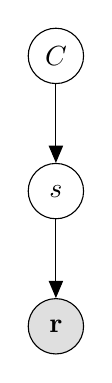
\begin{tikzpicture}
\node[obs]                               (r) {$\mathbf{r}$};
  \node[latent, above=of r] (s) {$s$};
   \node[latent, above=of s]  (c) {$C$};
   \edge {c} {s};
  \edge {s} {r}; 
 \end{tikzpicture}
 \\
$C$ is the category distribution ($\in \{0, 1\}$\\
$P(C) = .5$\\ 
$s$ is the presented stimulus, a draw from the selected category distribution\\
$P(s|C) = \mathcal{N} (s; 0, \sigma_{\text{C}}^2) = \mathcal{N} (s; 0, \tau_{\text{C}}^{-1})$\\
$\mathbf{r}$ is the vector of neural responses to $s$:
$P(r_i|s) = \text{Poisson}(r_i; f_i(s))$\\
~\\
$f_i(s)$ is the tuning curve of the $i^\text{th}$ neuron in response to a stimulus $s$\\
Tuning curve assumptions:
\begin{itemize}
\item Tuning curves cover the space so $\sum_i f_i(s)$ is independent of $s$
\item The tuning curves are Gaussian: $f_i(s) \sim \mathcal{N} (s_i^{\text{pref}}, \sigma_{\text{tc}}^2)$
\end{itemize}

\subsection{Inference}
\begin{equation}
\begin{aligned}
P(C, s|\mathbf{r}) &= \Big(\prod_i P(r_i|s)\Big) P(s|C) P(C)\\
&\propto \Big(\prod_i \text{Poisson}(r_i; f_i(s))\Big) \mathcal{N} (s; 0, \tau_{\text{C}}^{-1})\\
&= \Big(\prod_i \frac{f_i(s)^{r_i}}{r_i!} \Big) \sqrt{\frac{\tau_C}{2 \pi}} e^{\frac{-\tau_C s^2}{2}}
\end{aligned}
\end{equation}

Let 
\begin{equation}
\begin{aligned}
\tau_C &= \begin{cases}
\tau_0, & \text{if } C = 0\\
\tau_1, & \text{if } C = 1
\end{cases}\\
&= \tau_0 (1 - C) + \tau_1 C\\
&= \tau_0 = (\tau_0 - \tau_1)C\\
&= \tau_0 - C \Delta \tau
\end{aligned}
\end{equation}

For variational inference,
\begin{equation}
\begin{aligned}
\log P(C, s|\mathbf{r}) &= \sum_i \Big(- \log r_i! + r_i \log(f_i(s)) \Big) + \frac{-(\tau_0 - C \Delta \tau) s^2}{2} + \frac{1}{2} \log \Big(\frac{\tau_0 - C \Delta \tau}{2 \pi} \Big)
\end{aligned}
\end{equation}

\subsection{Variational approximation}
Then we approximate this using a factorized distribution:
\begin{equation}
Q(C, s|\mathbf{r}) = Q(C|\mathbf{r}) Q(s|\mathbf{r})
\end{equation}

\begin{equation}
\begin{aligned}
Q(C|\mathbf{r}) &= \langle \log P(C, s|\mathbf{r}) \rangle_{Q(s|\mathbf{r})}\\
&= \frac{-(\tau_0 - C \Delta \tau)}{2} \langle s^2 \rangle_{Q(s|\mathbf{r})} + \frac{1}{2} \log \Big(\frac{\tau_0 - C \Delta \tau}{2 \pi} \Big)\\
Q(s|\mathbf{r}) &= \langle \log P(C, s|\mathbf{r}) \rangle_{Q(C|\mathbf{r})}\\
&= \sum_i \Big(- \log r_i! + r_i \log(f_i(s)) \Big) + \frac{- (\tau_0 - \langle C \rangle_{Q(C|\mathbf{r})}  \Delta \tau)}{2} s^2
\end{aligned}
\end{equation}

\end{document}